\documentclass[a4paper,11pt]{article}
\usepackage{graphicx}
\usepackage{lscape}
\usepackage{capt-of}
\usepackage{fancyhdr}
\usepackage{caption}
\usepackage{subcaption}
\usepackage{tikz}
\usetikzlibrary{arrows.meta}
\usepackage{enumerate}
\usepackage{siunitx}
\usepackage{eurosym}
\usetikzlibrary{quotes,angles,positioning}
\usepackage{standalone}
\usepackage{multirow}

\usepackage{hyperref}
\hypersetup{
    colorlinks=true,
    linkcolor=blue,
    filecolor=magenta,      
    urlcolor=cyan,
}

\usepackage{geometry} % to change the page dimensions
\geometry{a4paper} 
\pagestyle{fancy}
\lhead{}
\rhead{Louis Carnec \\ 15204934}
\renewcommand{\headrulewidth}{0pt}
\setlength\parindent{0pt}
\usepackage{amstext} % for \text
\DeclareRobustCommand{\officialeuro}{%
  \ifmmode\expandafter\text\fi
  {\fontencoding{U}\fontfamily{eurosym}\selectfont e}}
\setlength{\parindent}{5ex}

\begin{document}



\begin{titlepage}

\newcommand{\HRule}{\rule{\linewidth}{0.5mm}} % Defines a new command for the horizontal lines, change thickness here

\center % Center everything on the page
 

%----------------------------------------------------------------------------------------
%	TITLE SECTION
%----------------------------------------------------------------------------------------

\HRule \\[0.4cm]
{ \huge \bfseries Network Software Modelling Assignment 2}\\[0.4cm] % Title of your document
\HRule \\[1.5cm]
 
%----------------------------------------------------------------------------------------
%	AUTHOR SECTION
%----------------------------------------------------------------------------------------

\begin{minipage}{0.4\textwidth}
\begin{flushleft} \large
\emph{Students:}\\
Louis \textsc{Carnec} \\% Your name
Vijay \textsc{Katta}\\
Adedayo \textsc{Adelowokan}  
\end{flushleft}
\end{minipage}
~
\begin{minipage}{0.4\textwidth}
\begin{flushright} \large
\emph{Student \#:} \\
15204934 \\ 15202724 \\15204151 % Supervisor's Name
\end{flushright}
\end{minipage}\\[4cm]

% If you don't want a supervisor, uncomment the two lines below and remove the section above
%\Large \emph{Author:}\\
%John \textsc{Smith}\\[3cm] % Your name

%----------------------------------------------------------------------------------------
%	DATE SECTION
%----------------------------------------------------------------------------------------

{\large \today}\\[3cm] % Date, change the \today to a set date if you want to be precise

%----------------------------------------------------------------------------------------
%	LOGO SECTION
%----------------------------------------------------------------------------------------

%\includegraphics{Logo}\\[1cm] % Include a department/university logo - this will require the graphicx package
 
%----------------------------------------------------------------------------------------

\vfill % Fill the rest of the page with whitespace

\end{titlepage}






\section{Read world phenomenon : Spread of disease through airports network} 


The world is closely connected than ever before, through transportation networks. Air, sea and land transportation continues to expand in reach, speed of travel and volume of passengers and goods carried. Pathogens and their vectors can now move further, faster and in greater numbers than ever before \cite{tatem2006global}. Epidemics can occur more easily and the emergence of novel pathogens exacerbates the situation \cite{jones2008global}. Understanding the dispersal behaviour and identifying the outbreak of an epidemic in the preliminary stages enables critical response planning. Network topology properties surrounding the debut location explains much of the early stage variation in the spread of diseases \cite{lawyer2016measuring}.

In this simulation we will model the spread of disease through world airports network. It is inspired by the work of Yager and Taylor \cite{nicholasyager2014} which models the spread of pathogens through airports using a directed graph. We extend their work of simulating disease spread by selectively infecting the nodes to analyse the impact of graph/node properties such as diameter, average path length , centrality and clustering. 

\section{Describe briefly your choice of graph model and how it corresponds to the real-world phenomenon, e.g. your choice of directed versus undirected edges, edge weights, allowing or disallowing self-loops, etc.}

Our real-world network graph is undirected where nodes represent airports and edges are routes.We used open source data from \href{http://openflights.org}{openflights.org} along with population of the cities. Redundant edges and unconnected nodes are removed from the graph. Average of population of two airpots is calculated and normalised and assigned as edge weight. Airports where both origin and destination are with-in USA are used, and others are removed.



\section{With the aid of a diagram, describe the simulation rules, e.g. how agents change state and what causes them to send messages.}



To simulate the propagation of a disease through the airports network, we have selected four states - susceptible, infected, recovered and  removed. Initial state of all nodes is susceptible and any node can be infected. There is no incubation period, a node once infected can infect neighbours with a probability of edge weight. An infected node recovers with a random probability which decreases as the number of steps increase. Alternatively a node with infection is removed from the network indefinitely. A node once infected and recovered is immune to infection and not susceptible any more.

Nodes are coloured based on the status - green is susceptible, yellow is infected, blue is recovered and red is removed/dead. Figure \ref{fig:M1} below has 5 blocks each one represents the status of nodes at one time step. Status of nodes in step 1 is shown by block \textit{(a)} , where node A is infected and is yellow , all the other nodes green showing that they are susceptible. In step 2 nodes B and D are infected with probabilities WAB and WDA respectively, as they are the neighbours of node A. Step 3 shows that all nodes are infected and in 4th time step, nodes B and D are red showing that they are dead/removed. Node C is blue in the last step representing that it has recovered from infection.


\begin{figure}[htbp]
\begin{subfigure}{.3\textwidth}
        \centering
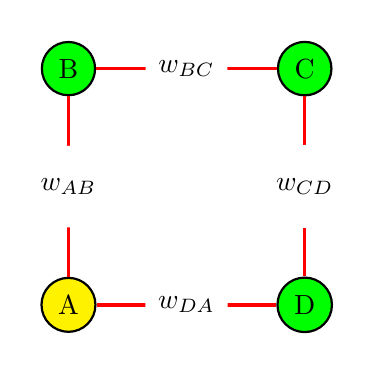
\begin{tikzpicture}
\begin{scope}[every node/.style={circle,thick,draw},local bounding box=aa]
    \node[fill = yellow] (A) at (0,0) {A};
    \node[fill = green] (B) at (0,3) {B};
     \node[fill = green]  (C) at (3,3) {C};
     \node[fill = green]  (D) at (3,0) {D};
\end{scope}

\begin{scope}[>={Stealth[black]},
              every node/.style={fill=white,circle},
              every edge/.style={draw=red,very thick}]
    \path [-] (A) edge node {$w_{AB}$} (B);
    \path [-] (B) edge node {$w_{BC}$} (C);
   \path [-] (C) edge node {$w_{CD}$} (D);
    \path [-] (D) edge node {$w_{DA}$}(A);
\end{scope}
\end{tikzpicture}
\caption{Initial node A infected}
        \label{fig:myfirstsubfig}
    \end{subfigure}%
\begin{subfigure}{.3\textwidth}
        \centering
        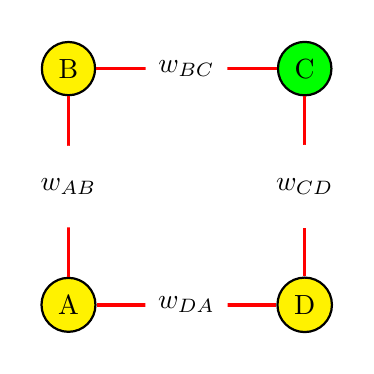
\begin{tikzpicture}
\begin{scope}[every node/.style={circle,thick,draw},shift={(4,0)},local bounding box=bb]
    \node[fill = yellow] (A) at (0,0) {A};
    \node[fill = yellow] (B) at (0,3) {B};
     \node[fill = green]  (C) at (3,3) {C};
     \node[fill = yellow]  (D) at (3,0) {D};
\end{scope}

\begin{scope}[>={Stealth[black]},
              every node/.style={fill=white,circle},
              every edge/.style={draw=red,very thick}]
    \path [-] (A) edge node {$w_{AB}$} (B);
    \path [-] (B) edge node {$w_{BC}$} (C);
   \path [-] (C) edge node {$w_{CD}$} (D);
    \path [-] (D) edge node {$w_{DA}$}(A);
\end{scope}
\end{tikzpicture}
        \caption{B and D infected}
        \label{fig:mysecondsubfig}
    \end{subfigure}
\begin{subfigure}{.3\textwidth}
        \centering
        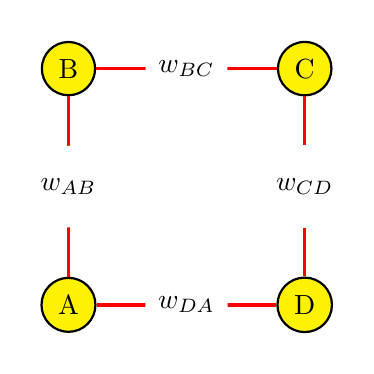
\begin{tikzpicture}
\begin{scope}[every node/.style={circle,thick,draw},shift={(8,0)},local bounding box=bb]
    \node[fill = yellow] (A) at (0,0) {A};
    \node[fill = yellow] (B) at (0,3) {B};
     \node[fill = yellow]  (C) at (3,3) {C};
     \node[fill = yellow]  (D) at (3,0) {D};
\end{scope}

\begin{scope}[>={Stealth[black]},
              every node/.style={fill=white,circle},
              every edge/.style={draw=red,very thick}]
    \path [-] (A) edge node {$w_{AB}$} (B);
    \path [-] (B) edge node {$w_{BC}$} (C);
   \path [-] (C) edge node {$w_{CD}$} (D);
    \path [-] (D) edge node {$w_{DA}$}(A);
\end{scope}
\end{tikzpicture}
        \caption{All nodes infected}
        \label{fig:mysecondsubfig}
    \end{subfigure}
    \begin{subfigure}{.4\textwidth}
        \centering
        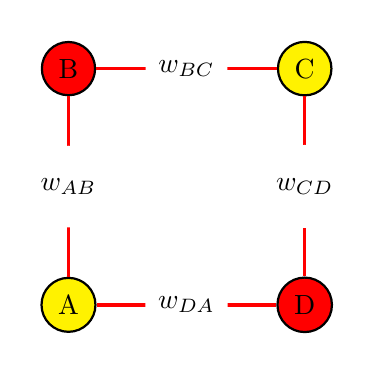
\begin{tikzpicture}
\begin{scope}[every node/.style={circle,thick,draw},shift={(8,0)},local bounding box=bb]
    \node[fill = yellow] (A) at (0,0) {A};
    \node[fill = red] (B) at (0,3) {B};
     \node[fill = yellow]  (C) at (3,3) {C};
     \node[fill = red]  (D) at (3,0) {D};
\end{scope}

\begin{scope}[>={Stealth[black]},
              every node/.style={fill=white,circle},
              every edge/.style={draw=red,very thick}]
    \path [-] (A) edge node {$w_{AB}$} (B);
    \path [-] (B) edge node {$w_{BC}$} (C);
   \path [-] (C) edge node {$w_{CD}$} (D);
    \path [-] (D) edge node {$w_{DA}$}(A);
\end{scope}
\end{tikzpicture}
        \caption{Infected nodes die after n steps}
        \label{fig:mysecondsubfig}
    \end{subfigure}
    \begin{subfigure}{.4\textwidth}
        \centering
        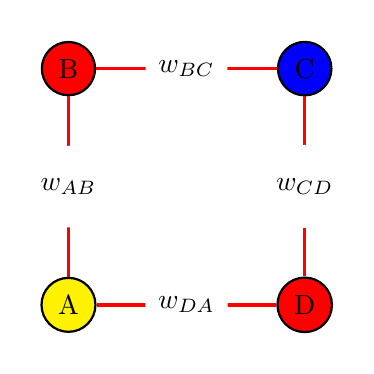
\begin{tikzpicture}
\begin{scope}[every node/.style={circle,thick,draw},shift={(8,0)},local bounding box=bb]
    \node[fill = yellow] (A) at (0,0) {A};
    \node[fill = red] (B) at (0,3) {B};
     \node[fill = blue]  (C) at (3,3) {C};
     \node[fill = red]  (D) at (3,0) {D};
\end{scope}

\begin{scope}[>={Stealth[black]},
              every node/.style={fill=white,circle},
              every edge/.style={draw=red,very thick}]
    \path [-] (A) edge node {$w_{AB}$} (B);
    \path [-] (B) edge node {$w_{BC}$} (C);
   \path [-] (C) edge node {$w_{CD}$} (D);
    \path [-] (D) edge node {$w_{DA}$}(A);
\end{scope}
\end{tikzpicture}
        \caption{Nodes C recovers}
        \label{fig:mysecondsubfig}
    \end{subfigure}

\caption{Spread of Infection Simulation Rules} \label{fig:M1}
\end{figure}
\section{Program your simulation in Python.}


\section{State one or more simulation properties which you wish to investigate and which graph properties you hypothesize they may depend on.}

As the size of the graph grows, it becomes increasingly difficult to visualise and understand it, thus quantitative performance measures are need. We will use the properties of graph/node such as Diameter and average path length,  Clustering, Centrality and Degree distributions, to analyse the impact of these metrics on the behaviour of the epidemic.

\paragraph{Diameter and average path length :} If \textit{l(u,v)} is the length of shortest path between nodes \textit{u} and \textit{v} , then the diameter of a graph(\textit{G}) is the largest distances between any two nodes in \textit{G}.

 \[ \textrm{diameter} = max \quad l(u,v ) \] 


The average path length is the average distance between any two nodes in the graph(\textit{G}). Maximum value of average path length is diameter, but can be much smaller than diameter. If the graph is not connected then the diameter is infinity, but for this study all unconnected nodes are removed from the graph. We hypothesise that airports graph with shorter diameter and average path length will result in the spread of the quicker.

\paragraph{Clustering :} Measures the extent to which a nodes' friends are friends with one another. This clustering measure is represented by the overall clustering
coefficient \textit{Cl(G)}, given by


 \[ Cl(G) = \frac{3* \textrm{number of triangles in the graph}}{\textrm{number of connected triples of nodes}}\] 
 

Another measure of clustering is defined for an individual node, it is given by 
 \[Cli (G ) = \frac{\textrm{number of triangles connected to node i} }{ \textrm{number of triples centered at i}}\] 

We hypothesise that graphs and nodes with high clustering coefficients will spread the disease quicker and are potential candidates that need intervention, to stop the disease from becoming an epidemic.

\paragraph{Centrality:} Importance of node's position in a graph is captured by the Centrality and there are different measures to do it.
\\Degree centrality: for node v of graph (G) with n nodes is given by,


 \[ \frac{d_{v} (G) }{n - 1} \textrm{, where } d_{v}(G) \textrm{, is the degree of node v}\] \\
 

Closeness centrality: Tracks how close a given node is to any other node: for node u, one such measure is given by 

 \[ \frac{n-1 }{\sum_{u \neq v} l(u,v) }  \textrm{ , where l(u, v) is the distance between u and v}  \]  \\
 
 Betweenness centrality: It measures the extent to which a node lies on paths between other nodes. If $n_{s,t}^{u}$ be the number of geodesic paths from $s$ to $t$ that pass through $u$ and let $n_{s,t}$ be the total number of geodesic paths from $s$ to $t$. Then the betweenness centrality of vertex $u$ is:

\[\displaystyle{b_u =  \sum_{s, t} \frac{n_{s,t}^{u}}{n_{s,t}}}\] \\

Nodes with high centrality tend to have considerable influence within a graph by virtue of their control over information passing between others. These nodes, when removed from the graph will most likely disrupt the spread of disease between other nodes as they lie on the largest number of routes.

\paragraph{Degree distributions:} The degree of a node is the number of neighbours of the node. For any integer $k \geq 0$, the quantity $p_k$ is the fraction of nodes having degree $k$. This is also the probability that a randomly chosen node in the graph has degree $k$. The quantities $p_k$, for $k \geq 0$, represent the degree distribution of the graph. 


\section{Carry out experiments to measure these properties in different types and sizes of graph (at least one real-world graph, and at least one scalable graph model such as the Erdos-Renyi random graph model, at multiple sizes). Present a table of data showing your results.}

Questions:

How quickly should a given country stop letting flights in to avoid the disease reaching it? when is too late? Different results for iceland and uk for example?...
Centrality of country: how quick does it get disease 

simulation property: screening for disease - catch given percentage -  effect on spread

simulation property - chance of receiving - centrality
probability of country with disease of spreading to other countries weighted on population of that country
probability increases at each timestep to account for fact that disease spreading within the country



Graph property tests - Tables of results

Results Diagrams/figures from Python code


Scalability  test results along with tables and figures

Diameter: airport graph - take subgraph (random vs high degree nodes vs low degree nodes) and compare rate of infection and effect on stats for 3 simulations. random graph - check for different pn

Shortest Path - pick 


\section{State your conclusions, based on your data.}

Discuss the results


Statistics

\clearpage

\bibliographystyle{acm}
\bibliography{NSM.bib}

\end{document}